\documentclass[10pt,twocolumn]{article}

\usepackage[a4paper,margin=0.75in]{geometry}
\usepackage{amsmath,amssymb}
\usepackage{booktabs}
\usepackage{graphicx}
\usepackage{microtype}
\usepackage{xcolor}
\usepackage[hidelinks]{hyperref}

\newcommand{\method}{\textsc{SERVIS}}
\newcommand{\SEthree}{\mathrm{SE}(3)}
\newcommand{\Tworldcam}{\mathbf{T}_{\mathrm{world}\leftarrow\mathrm{cam}}}
\newcommand{\todo}[1]{\textcolor{red}{[TODO: #1]}}

\title{\method: Evaluating Virtual Visual Servoing Across\\
Scene Representations and Image Error Signals}
\author{Anonymous authors}
\date{}

\begin{document}
\maketitle

\begin{abstract}
Camera relocalization can be formulated as analysis by synthesis: render a
scene from a pose hypothesis, compare the render with a target image, and
iteratively update the virtual camera. This paper presents \method, a common
experimental framework for studying how the image error signal and scene
representation affect that optimization. We compare dense photometric error
with keypoint-based error while holding the guarded Levenberg--Marquardt update
on $\SEthree$ fixed, and evaluate mesh, neural radiance field (NeRF), and 3D
Gaussian Splatting (3DGS) renderers. Experiments use the Stanford RGB Camera
Relocalization Dataset and report rotation and translation error, convergence
rate, iteration count, and wall-clock time. This source is a reproducible paper
draft; final aggregate results and statistical claims remain to be inserted
after completion of the benchmark matrix.
\end{abstract}

\section{Introduction}

Visual servoing closes a control loop around image measurements
\cite{hutchinson1996tutorial}. In virtual visual servoing, the controlled
camera is a renderer: a target observation is localized by moving a virtual
camera until its synthesized view agrees with the observation. This makes
camera pose estimation a nonlinear analysis-by-synthesis problem. Its energy
landscape depends not only on the optimizer but also on the fidelity of the
scene representation and on how image disagreement is measured.

Modern scene models offer different trade-offs. Mesh rasterization is explicit
and geometrically interpretable, NeRF provides continuous view synthesis
\cite{mildenhall2020nerf}, and 3DGS provides high-fidelity real-time rendering
\cite{kerbl20233d}. Dense photometric objectives use all valid pixels but are
sensitive to appearance mismatch; sparse feature objectives can tolerate some
photometric change but depend on repeatable correspondences. Comparing methods
without controlling the remaining pipeline can therefore confound renderer,
error-signal, and optimizer effects.

\method{} addresses this issue with one camera convention, depth gateway,
optimizer, stopping policy, dataset protocol, and metric implementation. The
study is organized around two controlled factors:

\begin{itemize}
  \item the error signal: dense photometric error or feature-based image error;
  \item the renderer: mesh, NeRF, or 3DGS.
\end{itemize}

The working hypothesis is that photometric optimization benefits most from
3DGS appearance fidelity. The benchmark is designed to test rather than assume
that hypothesis.

\section{Related Work}

Image-based visual servoing maps image residuals to camera motion through an
interaction matrix \cite{hutchinson1996tutorial}. Classical formulations use
geometric image features, while direct methods minimize intensity residuals.
Both are local estimators and depend on initialization, visibility, depth, and
the conditioning of the image Jacobian.

NeRF represents a scene with a learned volumetric radiance field
\cite{mildenhall2020nerf}. 3DGS instead represents it with anisotropic Gaussian
primitives and a differentiable tile-based rasterizer
\cite{kerbl20233d}. Although both support novel-view synthesis, their rendered
appearance, depth behavior, latency, and failure modes differ from those of a
mesh. These differences may directly alter the visual-servo energy landscape.

The Stanford RGB Camera Relocalization Dataset was introduced for large-scale
RGB and RGB-D relocalization \cite{valentin2016learning}. Its multi-sequence,
globally aligned camera poses make it suitable for testing iterative pose
refinement across large indoor rooms.

\section{Method}

\subsection{Pose and rendering loop}

The state is the camera-to-world transform $\Tworldcam\in\SEthree$, stored in
the OpenCV camera convention (right, down, forward). At iteration $k$, renderer
$\mathcal{R}$ produces color and depth from the current pose,
\begin{equation}
  (I_k, D_k) = \mathcal{R}(\mathbf{T}_k, \mathbf{K}, \mathcal{S}),
\end{equation}
where $\mathbf{K}$ contains intrinsics and $\mathcal{S}$ is the scene
representation. The controller constructs a residual $\mathbf{r}_k$ and
Jacobian $\mathbf{J}_k$, solves for a twist $\boldsymbol{\xi}_k\in\mathbb{R}^6$,
and updates the pose on $\SEthree$:
\begin{align}
  (\mathbf{J}_k^\top\mathbf{W}_k\mathbf{J}_k + \lambda_k\mathbf{D}_k)
  \boldsymbol{\xi}_k
    &= -\mathbf{J}_k^\top\mathbf{W}_k\mathbf{r}_k, \\
  \mathbf{T}_{k+1}
    &= \mathbf{T}_k\exp(\widehat{\boldsymbol{\xi}_k}).
\end{align}
Here $\lambda_k$ is the Levenberg--Marquardt damping term and
$\mathbf{W}_k$ encodes validity and robust weighting. Step guards reject
non-finite or implausibly large updates.

\subsection{Error signals}

For dense photometric servoing, the residual at valid pixel $\mathbf{u}$ is
\begin{equation}
  r_{\mathrm{photo}}(\mathbf{u}) =
  I_{\mathrm{target}}(\mathbf{u}) - I_k(\mathbf{u}).
\end{equation}
The image gradient, rendered depth, projection model, and camera-motion
interaction matrix form the Jacobian. Coarse-to-fine optimization enlarges the
practical basin of convergence.

For feature-based servoing, keypoints are detected and matched between the
target and rendered views. With matched normalized image coordinates
$\mathbf{x}^{t}_i$ and $\mathbf{x}^{r}_i$, the residual stacks
\begin{equation}
  \mathbf{r}_{\mathrm{feat}} =
  \left[\mathbf{x}^{t}_1-\mathbf{x}^{r}_1,\ldots,
  \mathbf{x}^{t}_N-\mathbf{x}^{r}_N\right]^\top.
\end{equation}
Depth is sampled at rendered keypoints, and invalid or geometrically
inconsistent matches are excluded before the same damped pose update.

\subsection{Depth policy}

Depth enters only through a single implementation boundary. The default is
metric monocular depth from MoGe2, without scale alignment. Renderer-intrinsic
depth is an explicit ablation. A requested estimator failure aborts the run;
the system never silently substitutes a different depth source. This policy
prevents an unreported depth change from contaminating comparisons.

\section{Experimental Protocol}

\subsection{Dataset}

We use the Stanford RGB Camera Relocalization Dataset
\cite{valentin2016learning}, available from
\url{https://graphics.stanford.edu/projects/reloc/}. It contains RGB-D data
from four large indoor scenes (Apartment 1, Apartment 2, Office 1, and Office
2), comprising 12 rooms. The captures pair a Structure depth sensor with an
iPad color camera. Each sequence includes RGB frames, millimetre depth, camera
calibration, and camera-to-world poses; sequences within a scene are globally
aligned by bundle adjustment.

For \method, each evaluated room is converted once to a common COLMAP-aligned
scene package. The image set and all renderer assets share the original world
frame. Mesh, 3DGS, and NeRF models are built from the same training split. Query
frames used for evaluation are excluded from renderer training.

\subsection{Controlled comparison}

The core matrix is shown in Table~\ref{tab:matrix}. Camera initialization,
intrinsics, resolution, optimizer safeguards, stopping rules, and evaluation
queries are held fixed within each comparison block.

\begin{table}[t]
  \centering
  \caption{Core experimental matrix. Every error signal is evaluated with
  every renderer under a shared protocol.}
  \label{tab:matrix}
  \small
  \begin{tabular}{@{}lll@{}}
    \toprule
    Factor & Levels & Held fixed \\
    \midrule
    Error & Photometric, feature & LM on $\SEthree$ \\
    Renderer & Mesh, NeRF, 3DGS & Camera/query set \\
    Depth & MoGe2, intrinsic & Explicit per run \\
    \bottomrule
  \end{tabular}
\end{table}

Initial poses are sampled at controlled rotation and translation offsets from
the reference camera. The exact random seeds, offset bins, frame list, renderer
checkpoints, and configuration files must accompany the final results.

\subsection{Metrics}

For estimate $\widehat{\mathbf{T}}$ and reference $\mathbf{T}^{*}$, translation
error is the Euclidean distance between camera centers. Rotation error is the
geodesic angle
\begin{equation}
  e_R = \cos^{-1}\!\left(\frac{\operatorname{tr}
  (\widehat{\mathbf{R}}^\top\mathbf{R}^{*})-1}{2}\right).
\end{equation}
We report final rotation error in degrees, translation error in metres,
convergence rate under a predeclared joint threshold, iterations to termination,
and end-to-end wall-clock time. Aggregate results include medians and dispersion
across queries and initialization bins, not only successful trials.

\section{Results and Analysis}

Figure~\ref{fig:representations} illustrates qualitative RGB and depth
differences among the three scene representations. The panels motivate the
central measurement question: higher RGB fidelity need not imply equally
reliable depth for control.

\begin{figure}[t]
  \centering
  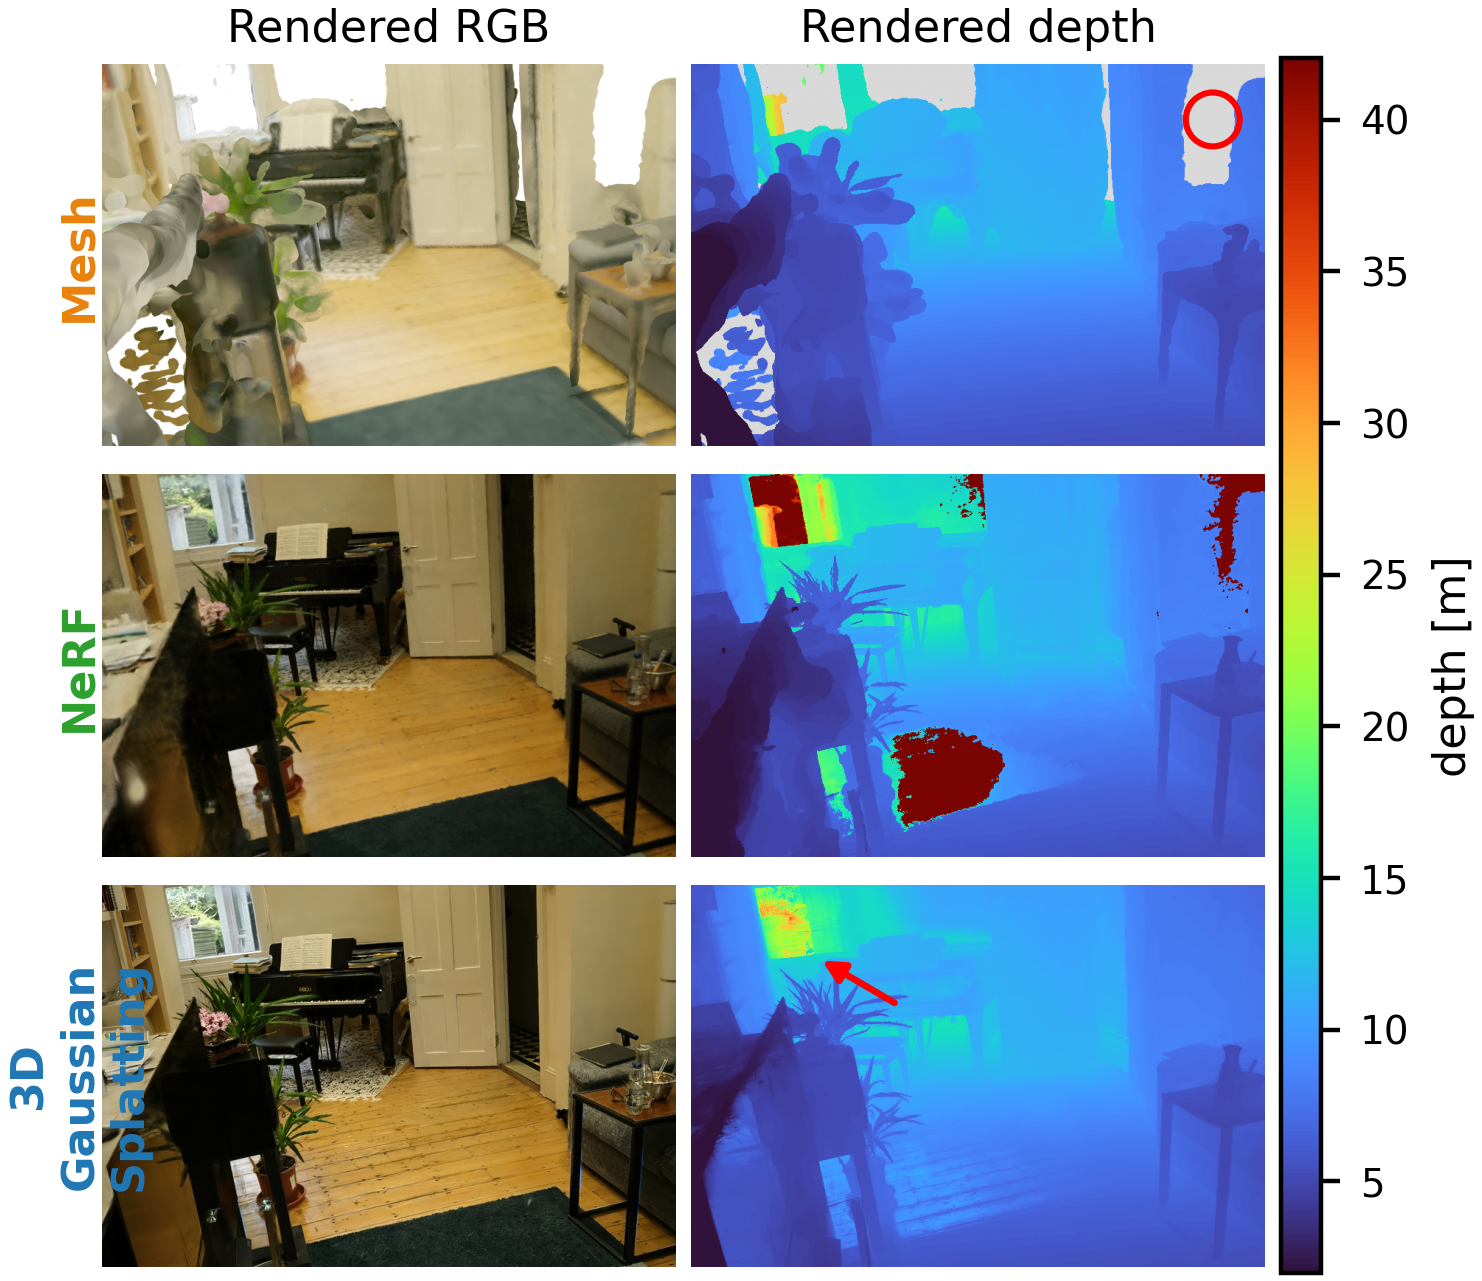
\includegraphics[width=\columnwidth]{figures/fig1_repr_room.png}
  \caption{Representative rendered RGB and depth from mesh, NeRF, and 3DGS.
  Red annotations identify depth artifacts relevant to the interaction matrix.}
  \label{fig:representations}
\end{figure}

Figure~\ref{fig:case-study} records an observed 3DGS depth/downsampling case
study. It is retained as a diagnostic example and must not substitute for the
aggregate benchmark.

\begin{figure}[t]
  \centering
  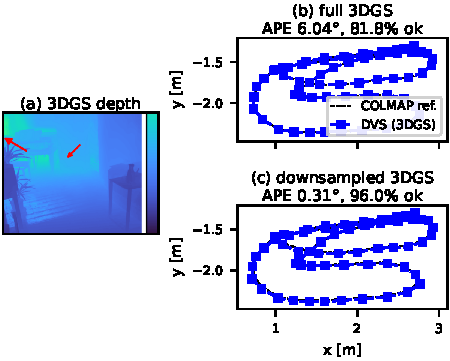
\includegraphics[width=\columnwidth]{figures/fig2_case_study.pdf}
  \caption{Diagnostic case study relating 3DGS depth artifacts and image
  downsampling to trajectory absolute pose error (APE).}
  \label{fig:case-study}
\end{figure}

\begin{figure}[t]
  \centering
  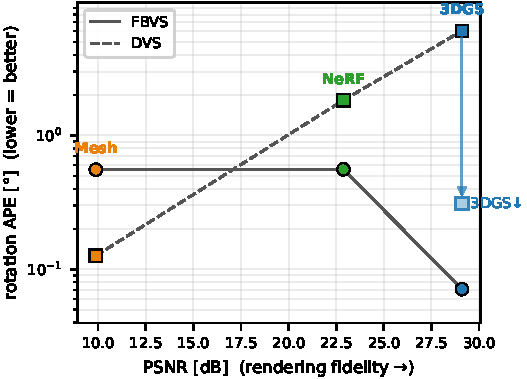
\includegraphics[width=\columnwidth]{figures/fig3_fidelity_control.pdf}
  \caption{Draft view of rendering fidelity versus rotation APE for
  feature-based visual servoing (FBVS) and dense visual servoing (DVS). The
  final paper will replace this summary with results generated by the frozen
  benchmark protocol.}
  \label{fig:fidelity}
\end{figure}

The final analysis will answer the following questions:
\begin{enumerate}
  \item Which renderer/error pair has the highest convergence rate?
  \item How do final pose accuracy and convergence basin change with initial
        offset?
  \item Does novel-view fidelity predict pose accuracy for both controllers?
  \item What accuracy--latency trade-off does each renderer impose?
  \item Which failures arise from appearance, matching, or depth artifacts?
\end{enumerate}

\todo{Insert the frozen benchmark table, confidence intervals, hardware and
software versions, and per-room results.}

\section{Limitations}

The study evaluates local pose refinement and therefore does not by itself
solve global place recognition. Renderer training quality, scene coverage, and
pose initialization constrain the observed convergence basin. Dense objectives
remain vulnerable to exposure changes and non-Lambertian effects, while sparse
objectives depend on detector repeatability. Monocular and renderer-derived
depth have different failure modes and must be reported separately. Finally,
the Stanford dataset is indoor and captured with a particular RGB-D rig, so
conclusions may not transfer unchanged to outdoor or strongly dynamic scenes.

\section{Conclusion}

\method{} provides a controlled framework for isolating the effects of scene
representation and image error signal in virtual visual servoing. The final
paper will report the complete mesh/NeRF/3DGS by photometric/feature matrix on
the Stanford RGB Camera Relocalization Dataset and test whether appearance
fidelity translates into a larger, faster, and more accurate pose-convergence
basin.

\bibliographystyle{plain}
\bibliography{references}

\end{document}
